\documentclass[11pt,a4paper]{article}
\usepackage[margin=25mm]{geometry}
\usepackage{newtxtext}
\usepackage[T1]{fontenc}
\usepackage[utf8]{inputenc}
\usepackage{microtype,graphicx,booktabs,longtable,amsmath,amssymb,amsthm,array,xspace}
\usepackage[round,authoryear]{natbib}
\usepackage[colorlinks=true,allcolors=blue]{hyperref}
\usepackage{fancyhdr}
\pagestyle{fancy}\fancyhf{}
\fancyhead[L]{\small HyperGranular-RAG: evidence completion}
\fancyhead[R]{\small Journal manuscript}
\fancyfoot[C]{\thepage}
\setlength{\headheight}{14pt}
\setlength{\parskip}{3pt}
\newtheorem{proposition}{Proposition}
\newtheorem{example}{Example}
\newcommand{\hgrag}{HyperGranular-RAG\xspace}
\newcommand{\full}{\textsc{Full}\xspace}
\newcommand{\effHotpot}{+0.01478}
\newcommand{\ciHotpot}{[0.00020,\,0.02988]}
\newcommand{\effMusique}{+0.01140}
\newcommand{\ciMusique}{[0.00450,\,0.01835]}
\newcommand{\effGemma}{+0.00516}
\newcommand{\ciGemma}{[-0.00262,\,0.01295]}
\newcommand{\effJoint}{+0.01357}
\newcommand{\ciJoint}{[0.00491,\,0.02233]}
\newcommand{\effFacet}{+0.01336}
\newcommand{\ciFacet}{[0.00341,\,0.02343]}
\newcommand{\effProtection}{+0.00354}
\newcommand{\ciProtection}{[-0.00675,\,0.01389]}
\newcommand{\effStrong}{-0.03998}
\newcommand{\ciStrong}{[-0.05393,\,-0.02621]}
\newcommand{\effBm}{-0.00755}
\newcommand{\ciBm}{[-0.02259,\,0.00773]}
\newcommand{\effHybrid}{-0.00320}
\newcommand{\ciHybrid}{[-0.01591,\,0.00942]}
\newcommand{\effSidecar}{-0.00256}
\newcommand{\ciSidecar}{[-0.00998,\,0.00458]}
\newcommand{\effSidecarFacet}{-0.00743}
\newcommand{\ciSidecarFacet}{[-0.01616,\,0.00132]}
\newcommand{\effSidecarPlace}{+0.01122}
\newcommand{\ciSidecarPlace}{[0.00129,\,0.02104]}
\newcommand{\effSidecarUnprotected}{-0.01379}
\newcommand{\ciSidecarUnprotected}{[-0.02440,\,-0.00339]}
\newcommand{\effNative}{-0.00305}
\newcommand{\ciNative}{[-0.00688,\,0.00063]}
\newcommand{\effNativeFacet}{+0.00063}
\newcommand{\ciNativeFacet}{[-0.00422,\,0.00536]}
\newcommand{\effNativePlace}{+0.00337}
\newcommand{\ciNativePlace}{[-0.00129,\,0.00803]}
\newcommand{\effNativeUnprotected}{-0.00641}
\newcommand{\ciNativeUnprotected}{[-0.01171,\,-0.00118]}

\title{HyperGranular-RAG: Benefits and Boundaries of\\
Structured Evidence Completion in Multi-Hop Question Answering}
\author{Anonymous authors}
\date{}
\begin{document}
\maketitle
\begin{abstract}
Evidence selection for multi-hop retrieval-augmented generation is a joint
coverage problem constrained by an evidence-list budget. A relevant sentence can
still be insufficient without a complementary bridge, yet introducing that
bridge may displace useful context. This article examines structured evidence
completion through \hgrag: a geometry-based organization of candidate
sentences, a seed-relative facet-hyperedge selector, and a bounded insertion
policy that protects the beginning of a dense ranking.
We consolidate the historical compact, cross-space sidecar, and BGE-native
implementations while keeping their data boundaries distinct. Independent
dataset-canonical rescoring preserves every confirmation estimate.
With Qwen2.5-1.5B-Instruct, compact completion improves answer F1
over MiniLM Dense by $0.01478$, $0.01140$, and $0.01357$ in three
closed-candidate HotpotQA and MuSiQue evaluations; the recorded 95\%
paired bootstrap intervals exclude zero. The specified compact facet
selector also exceeds a centroid-only alternative. In contrast, the original
compact system falls below BGE, and neither tested BGE extension establishes
an increment over that baseline. Generator transfer remains unresolved.
Protected placement exceeds front insertion with identical visible evidence
in the cross-space study. We relate these outcomes to supporting-evidence
turnover and the distinction between group-level facets and prompt-visible
coverage. Analytical clarification shows why increased granular-ball compactness
alone is not evidence of semantic improvement and why heuristic expansion
cannot inherit an answer-quality guarantee from a coverage surrogate.
The resulting account identifies a useful compact-backbone intervention and
the empirical and theoretical limits of that intervention, without treating
later synthetic prototypes as evaluated methods.
\end{abstract}
\noindent\textbf{Keywords:} retrieval-augmented generation; multi-hop question
answering; evidence selection; granular representations; uncertainty.

\section{Introduction}
Retrieval-augmented question answering depends on two distinct capabilities:
finding relevant information and supplying a generator with a usable
combination of that information. A strong relevance ranking addresses the
first capability, but does not necessarily satisfy the second. For a question
requiring an entity bridge, several highly relevant sentences about the first
entity may be less useful than one additional sentence connecting it to the
second. Dense retrieval \citep{karpukhin2020dpr} provides a natural backbone
for this process, while multi-hop benchmarks expose the need to assemble
related facts \citep{yang2018hotpotqa,trivedi2022musique}.

A finite evidence-list budget makes completion a replacement decision. If a system
retains at most twenty evidence units, moving an additional candidate into the
context can remove another unit. The new item may increase annotated support
coverage without improving the answer; it may also duplicate retained
evidence or move information to a position the generator uses poorly.
Position-sensitive context use has been documented in language models
\citep{liu2024lostmiddle}. Consequently, the number of retrieved supporting
facts, their placement, and the answer produced from them are related but
non-interchangeable outcomes.

\hgrag studies a bounded intervention on this ranking. Candidate sentence
embeddings are organized into local granular balls. Query terms define facets
over these balls, and seed-relative facet hyperedges identify candidate
regions that differ from the initial seeds. A placement policy retains the
first ten dense entries and supplies at most four candidates before filling
the remaining positions from the dense order. The method is an
evidence-completion layer: it preserves a retrieval backbone and does not
replace corpus search with a learned graph model.

This article asks four connected questions. First, can structured completion
improve a compact dense retriever on end-to-end answers? Second, which of the
available component comparisons support that improvement? Third, does the
increment persist when the primary ranking is supplied by BGE? Fourth, what
do evidence-turnover and geometric analyses explain about the observed
boundary? These questions organize the presentation, rather than the
chronology of implementation and evaluation.

The empirical answer is conditional. Across three Qwen evaluations, the
historical compact implementation improves over MiniLM Dense. In the joint
component study, the facet-conditioned selector exceeds the specified
centroid-only control. Nevertheless, the original compact system is worse
than BGE. Adding compact candidates to BGE and rebuilding the structure in
BGE space both produce intervals crossing zero. The positive compact effects
therefore establish a capability within that system, while the BGE results
limit claims about general retrieval improvement.

The interpretation requires precise versioning. The historical compact
selector computes scores once relative to the seeds, rather than recomputing
true coverage marginals after every selection. Its recorded radius threshold
does not independently trigger a split under the frozen size constraints.
BGE-native reconstruction also changes geometry and scoring, so it is not
an encoder-only substitution. Later engineering repairs and synthetic dynamic
prototypes are not sources of the historical answer-quality results.

Our contribution is a complete, bounded empirical account of structured
completion, accompanied by definitions that make its mechanisms testable.
We provide the historical algorithms and their distinct comparisons;
consolidate positive, negative, and unresolved answer-quality effects;
connect candidate addition to evidence displacement and verified ordering
effects; and clarify geometric and objective-function limits of possible
explanations. Standard compactness identities and the coverage bound are
background tools, not new theoretical contributions. The extended analysis
uses existing results and mathematical reasoning, not new answer-quality
experiments. It does not establish that granular balls are indispensable or
that facet hyperedges outperform all simpler diversity and coverage rules.

\section{Positioning within Retrieval and Evidence Selection}
\subsection{From Relevance Ranking to Connected Retrieval}
Dense passage retrieval learns query and passage encoders for relevance
matching \citep{karpukhin2020dpr}. Multi-hop retrieval introduces dependencies
between retrieval steps. MDR conditions a subsequent retrieval on preceding
evidence \citep{xiong2021mdr}, whereas IRCoT alternates retrieval with generated
reasoning \citep{trivedi2023ircot}. Those methods change how a system reaches
evidence. Our closed-candidate intervention instead changes which already
available units enter a bounded context.

This distinction determines the scope of evaluation. A method can improve
selection from a supplied candidate set without improving first-stage corpus
recall. Conversely, a corpus retriever can reach the correct document without
selecting the sentence the generator needs. The present study addresses the
second type of problem conditional on candidate availability. It therefore
does not claim to solve open-domain reachability.

\subsection{Structure at Different Representational Levels}
RAPTOR constructs a hierarchy through recursive abstraction
\citep{sarthi2024raptor}. HippoRAG uses knowledge-graph structure and
propagation \citep{gutierrez2024hipporag}. HyperGraphRAG encodes n-ary
knowledge using hypergraph-structured representation
\citep{luo2025hypergraphrag}. These methods differ in the object being
organized, how relations are produced, and how the structure is traversed.
Their results cannot be imported as measurements under our generator and
evidence budget.

In \hgrag, a granular ball is a local group of sentence embeddings with a
center and radius, inspired by granular representations
\citep{xia2019granularball}. A facet hyperedge relates seed balls to an
expansion ball through query-term coverage. This relation is not an asserted
real-world fact and does not result from an entity-relation extraction model.
The structure is query-local, computed from the available candidate set, and
used to rank a small expansion. The historical study contains no
budget-aligned direct comparison with RAPTOR, HippoRAG, or HyperGraphRAG.

\subsection{Coverage and Diversity as Alternative Explanations}
A structured selector may improve a ranking simply by avoiding redundant
evidence. MMR is a classical relevance--redundancy rule
\citep{carbonell1998mmr}. Explicit coverage and diversity objectives can offer
another route to evidence selection \citep{lin2011submodular}.
These alternatives matter because a useful grouping heuristic does not by
itself establish that high-order relations caused the benefit.

We use the term \emph{facet-conditioned} to describe the implemented rule,
not to settle that causal question. Its compact NoFacet comparison replaces
the selector with centroid-only ball expansion. It does not hold every
possible coverage or diversity principle constant, and it does not compare
the method to a sentence-level coverage optimizer. The distinction between
a pipeline comparison and a pure component intervention is maintained
throughout the analysis.

\subsection{Context Use and Empirical Uncertainty}
Long-context evaluations show that evidence location can affect model
performance \citep{liu2024lostmiddle}. This motivates protecting an initial
retrieval prefix, but does not prove that ten entries is an optimal protection
budget. Likewise, statistical testing guidance emphasizes the relationship
between a statistic, a null hypothesis, and the dependence structure of the
sample \citep{dror2018hitchhiker}. We report historical estimates with their
recorded intervals and describe the evaluator and inferential caveats
explicitly, rather than strengthening a result through terminology.

\section{Problem Definition and Historical Algorithms}
\subsection{Candidate, Ranking, and Prompt Spaces}
Let $q$ denote a question and $U_q$ the finite set of sentence units supplied
by its benchmark context. A unit includes a document title, sentence text,
and a stable identity. The encoder receives the title and sentence, and
produces a normalized embedding $\hat e_u$. With query embedding $\hat e_q$,
the dense relevance score is
\begin{equation}
s(q,u)=\hat e_q^\top\hat e_u.
\end{equation}
Units are ordered by decreasing score and increasing identity. The baseline
list $D_q$ contains the first $K_q=\min(20,|U_q|)$ unique units.
The completed list $R_q$ has the same length.

Three evidence objects must be distinguished. The \emph{candidate insertion
set} contains units accepted by an expansion policy. The \emph{final ranking}
is the ordered list after placement, deduplication, and truncation to $K_q$.
The \emph{prompt-visible evidence} is the text actually retained by the
token-limited prompt. Equality at one level does not automatically imply
equality at the next. In particular, a fixed number of sentence units is not
a fixed number of tokens.

\subsection{Compact Granular-Ball Organization}
The compact method uses MiniLM embeddings for both relevance and grouping.
It begins with the whole candidate set as one root. For a ball $B$,
\begin{equation}
c_B=\operatorname{norm}\left(\sum_{u\in B}\hat e_u\right),\quad
d(u,B)=1-\hat e_u^\top c_B,\quad r_B=\max_{u\in B}d(u,B).
\end{equation}
Compactness is $C(B)=1-|B|^{-1}\sum_{u\in B}d(u,B)$.
The historical split eligibility rule is
\begin{equation}
\operatorname{depth}(B)<6\quad\land\quad |B|\geq4
\quad\land\quad (|B|>3\ \lor\ r_B>0.78).
\label{eq:split}
\end{equation}
Because $|B|\geq4$ implies $|B|>3$, the radius disjunction is inactive.
The first split seed is farthest from the center; the second has minimum
cosine similarity to the first. Assignment uses the more similar seed and
the frozen tie rule. A split is accepted only when each child has at least
two members. Otherwise the unsplit group becomes a leaf, possibly with more
than three members.

Thus the historical partition adapts to size and geometry, but is not
independently radius-triggered. We retain its actual definition rather than
replacing the predicate and attributing old results to a revised algorithm.
The compactness analysis in Section~\ref{sec:theory} explains why geometrically
more compact children are not, on their own, validated semantic evidence units.

\subsection{Facet Hyperedges and Static Selection}
The fixed tokenizer extracts ASCII-alphanumeric content terms and removes
the recorded stop words. Let $T_q$ denote query terms and
$T_B=T_q\cap\bigcup_{u\in B}T(u)$ the facets of ball $B$, using its title and
sentence text. The two balls with highest query--centroid similarity are the
seeds. Their union of facets, $T_{\mathrm{seed}}$, defines the reference for
expansion.

For a non-seed ball, write
$n_B=|T_B\setminus T_{\mathrm{seed}}|$,
$t_B=|T_B|$, $m=|T_q|$,
$b_B=\hat e_q^\top c_B$,
$a_B=\max_{S\in\mathrm{seeds}}c_B^\top c_S$, and
$\rho_B=|T_B\cap T_{\mathrm{seed}}|/|T_B|$ when $T_B$ is nonempty.
The candidate score is
\begin{equation}
h_B=.45\frac{n_B}{\max(m,1)}+.20\frac{t_B}{\max(m,1)}
     +.20b_B+.15(1-a_B)-.20\rho_B-.05|B|/8.
\label{eq:compactscore}
\end{equation}
Eligibility requires $n_B\geq1$, $|B|\leq8$, $b_B\geq.12$ or $a_B\geq.05$,
$|B|/n_B\leq6$, $\rho_B\leq.90$, and $h_B\geq.10$.
Eligible balls are ordered by decreasing $h_B$ and stable edge identity; at
most two distinct expansion balls are selected. Their units retain dense-score
and identity order. The historical unit-level facet bonus is zero.

A facet hyperedge is the relation between the seed balls and an eligible
expansion ball contributing seed-relative new facets. It identifies a region
of candidates; it does not assert that every unit in that region supplies the
missing fact. All eligibility and score calculations occur once. Updating an
internal covered-term set after accepting a ball does not recompute the
remaining scores. This static rule is different from true marginal-coverage
greedy selection.

\subsection{Protected Bounded Insertion}
Let $P_q$ be the first $\min(10,K_q)$ entries of $D_q$. The compact method
traverses the expansion order, skips duplicates in $P_q$, and accepts at most
four units with dense score at least $0.1957079917192459$. The floor is a
historical development-calibrated 25th percentile, transferred unchanged.
It is not a percentile recomputed on each evaluation set.
The policy concatenates the protected prefix, accepted units, and remaining
dense entries, applies stable deduplication, and truncates to $K_q$.

An accepted unit can already be in dense positions 11--20. Such an event is
a promotion within the baseline set; it differs from introducing a new unit
outside that set. Both consume placement capacity. This distinction matters
when interpreting insertion counts as evidence expansion. Candidate counts
cannot be substituted for counts of genuinely new supporting facts.

\begin{figure}[t]
\centering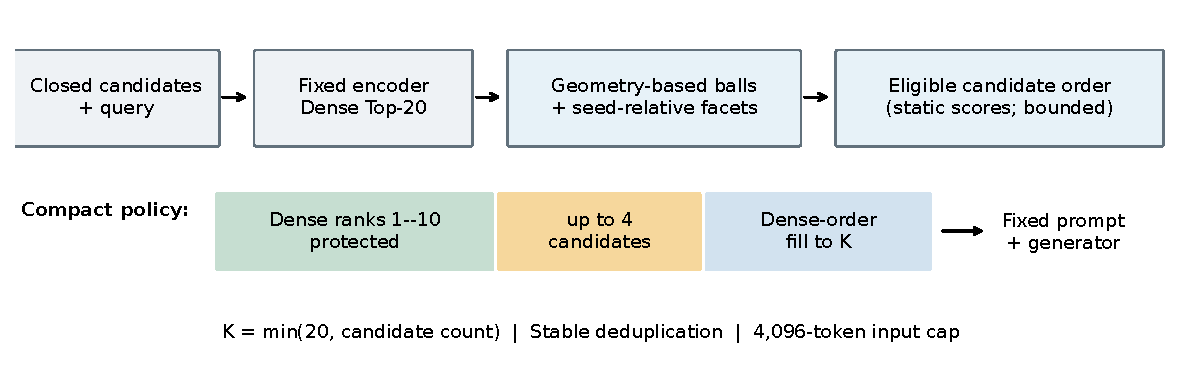
\includegraphics[width=\textwidth]{../shared/workflow.pdf}
\caption{Historical compact completion. The root includes the full candidate
pool. Static facet selection precedes placement; final list length and the
generator's token cap are separate constraints. This diagram depicts the
historical implementation, not the unexecuted dynamic prototype.}
\label{fig:workflow}
\end{figure}

\subsection{Cross-Space Sidecar}
The sidecar holds BGE's dense ranking as the reference while the frozen
MiniLM structure proposes eligible units outside BGE Top-20. It introduces
no learned score fusion. Protected placement inserts its accepted candidates
after the BGE prefix; unprotected placement puts the same candidates first.
Both then fill from BGE and enforce the same effective list length.

The sidecar asks whether a compact structure contains useful complementary
evidence that BGE does not already expose. It is more targeted than comparing
the original MiniLM pipeline against BGE, because the primary ranking now
comes from BGE in both arms. It remains a cross-space construction: the
candidate source and its score geometry are not native to BGE.

\subsection{BGE-Native Reconstruction}
The native implementation changes that geometry. A separate development
family crosses leaf target $\{4,6\}$, insertion budget $\{2,4\}$,
unit-score percentile floor $\{.50,.75\}$, and broad/strict facet gates,
giving 16 configurations. The selected C10 uses leaf target six, budget four,
floor $.50$, and broad gates. The confirmation comparison fixes that choice.

Native splits use depth limit eight, minimum child fraction $.20$, and a
weighted-child compactness improvement greater than $10^{-10}$. Seed
selection uses deterministic center-relative two-seed geometry and identity-based ties.
Within a query, unit relevance, ball relevance, radius, compactness, and
density are converted to empirical percentiles, where the percentile of a
value is the fraction of values less than or equal to it. Density is group
size divided by radius with the recorded small denominator floor.

Two seed balls are selected by relevance percentile, density percentile, and
identity. Broad gates require ball-relevance percentile at least $.35$ and
density percentile at least $.25$; strict gates use $.50$ for both.
Eligible expansion balls must have a seed-relative new facet and are ranked by
\begin{equation}
h_B^{N}=.55p_B+.25p_{\rho,B}+.15p_{C,B}
        +.05\min(n_B,3)/3.
\end{equation}
At most four balls supply units. A candidate must be outside BGE Top-20 and
meet the configured unit percentile floor. Its score is
\begin{equation}
h_u^{N}=.45p_u+.25p_B+.15p_{\rho,B}+.10p_{C,B}
        +.05\min(n_B,3)/3.
\end{equation}
Native NoFacet removes the new-facet gate and uses
$.50p_u+.30p_B+.10p_{\rho,B}+.10p_{C,B}$ for units.
It therefore changes several coefficients as well as facet eligibility.
Its result is a pipeline contrast, not a coefficient-preserving pure ablation.
The native study cannot be read as changing only the encoder in the compact
algorithm.

\section{Analytical Properties and Their Limits}
\label{sec:theory}
\subsection{Compactness Is a Resultant-Length Statistic}
The following properties concern the mathematical representation. They are
not claims about new empirical performance.
\begin{proposition}
For nonempty $B$ with unit embeddings $x_i$, and nonzero
$s_B=\sum_{i\in B}x_i$, the historical mean-cosine compactness satisfies
\begin{equation}
C(B)=\frac{1}{|B|}\sum_{i\in B}x_i^\top\frac{s_B}{\|s_B\|}
     =\frac{\|s_B\|}{|B|}\in[0,1].
\end{equation}
The scalar has the continuous extension $C(B)=0$ at $s_B=0$.
\end{proposition}
\begin{proof}
Linearity of the inner product gives
$\sum_i x_i^\top s_B/\|s_B\|=s_B^\top s_B/\|s_B\|=\|s_B\|$.
The upper bound follows from $\|\sum_i x_i\|\leq\sum_i\|x_i\|=|B|$.
Continuity follows from continuity of the norm.
\end{proof}
The scalar extension does not determine a normalized center at zero.
The compact implementation's zero-vector convention and the native
implementation's fallback direction can consequently have different
assignment behavior even though the exact zero-sum scalar is the same.

\begin{proposition}
For every partition $B=\bigsqcup_{j=1}^m B_j$ into nonempty groups,
\begin{equation}
\sum_j\frac{|B_j|}{|B|}C(B_j)\ \geq\ C(B).
\label{eq:partition}
\end{equation}
\end{proposition}
\begin{proof}
Writing $s_j=\sum_{i\in B_j}x_i$, the left side is
$|B|^{-1}\sum_j\|s_j\|$, while the right side is
$|B|^{-1}\|\sum_j s_j\|$. The triangle inequality gives the claim.
\end{proof}
Equality holds when the nonzero group sums share a direction. Otherwise a
strict increase can arise without any semantic alignment. For four
orthogonal unit vectors, parent compactness is $1/2$; every partition into
two pairs has weighted compactness $1/\sqrt{2}$. A positive compactness change
is therefore not evidence that a split recovered a reasoning relation.
The native balance and depth rules constrain a procedure, but do not change
this logical limitation.

\subsection{Scalar Stability Does Not Guarantee Partition Stability}
For corresponding perturbed vectors $x'_i$, the reverse triangle inequality
yields
\begin{equation}
|C'(B)-C(B)|\leq\frac{\|\sum_i(x'_i-x_i)\|}{|B|}
\leq\frac{1}{|B|}\sum_i\|x'_i-x_i\|.
\end{equation}
This is a stability bound for the scalar with membership fixed. It does not
bound changes in the normalized center near a zero sum, nor does it keep
discrete assignments fixed. For example, $x_1=(1,0)$ and
$x_2=(-1,\epsilon)/\sqrt{1+\epsilon^2}$ have a sum whose direction approaches
the positive vertical axis as $\epsilon\downarrow0$. Replacing $\epsilon$
with $-\epsilon$ makes the input perturbation arbitrarily small while
reversing that limiting direction. A stability claim for a full partition
would need additional separation assumptions.

\subsection{Seed-Relative Novelty Is Not a Dynamic Marginal}
Suppose seeds cover $\{\alpha\}$ and three candidate groups cover
$\{\beta\}$, $\{\beta\}$, and $\{\gamma\}$. A static score order can select
the first two. Both were new relative to the seeds, but the second adds no
facet after the first is selected. A dynamic coverage rule would reconsider
the remaining candidates at that point. This is a structural difference
between algorithms, not an estimate of how often the event occurs in the
historical corpus.

Likewise, let a selected group contain two sentences with facets
$\{\alpha\}$ and $\{\beta\}$, while the placement rule emits only the first.
The group union is $\{\alpha,\beta\}$ but selected-unit coverage is
$\{\alpha\}$. We call their difference \emph{phantom coverage}: a facet
credited to the group but absent from the selected units. Prompt truncation
can further reduce visible content. None of the historical aggregate results
measures the prevalence or answer effect of this particular discrepancy.

\subsection{A Coverage Guarantee Applies Only to Its Own Objective}
To make the distinction concrete, consider a fixed set of units, fixed
observable facets $T(u)$, and nonnegative weights $w_t$. Define
\begin{equation}
F(S)=\sum_t w_t\,\mathbf{1}\left[t\in\bigcup_{u\in S}T(u)\right].
\end{equation}
For a fixed protected set $P$, let $f_P(A)=F(P\cup A)-F(P)$.
The residual objective is normalized, monotone, and submodular: as $A$ grows,
the set of new facets available from any additional unit can only shrink.
This kind of explicitly specified coverage objective is consistent with the
objective-based approach discussed by \citet{lin2011submodular}.

If at most $b$ additional units are allowed and greedy selection recomputes
the true marginal each step, then for an optimal additional set $O$,
\begin{equation}
f_P(O)-f_P(A_i)\leq
\sum_{u\in O\setminus A_i}\big[f_P(A_i\cup\{u\})-f_P(A_i)\big]
\leq b\big[f_P(A_{i+1})-f_P(A_i)\big].
\end{equation}
Iterating gives
$f_P(A_b)\geq[1-(1-1/b)^b]f_P(O)\geq(1-1/e)f_P(O)$ for $b\geq1$.
The $b=0$ case is trivial, and selecting all remaining units is optimal if
fewer than $b$ are available.

This is the standard greedy coverage bound, specialized to an explicitly defined surrogate under a
cardinality budget and a fixed prefix. The historical static score in
Equation~\ref{eq:compactscore} does not implement that algorithm.
Variable token costs, negative penalties, changing facets, and generated
answer F1 are outside the statement. In particular, a coverage guarantee
cannot be used as an answer-quality guarantee.

\section{Empirical Design}
\subsection{Data Boundaries and Research Questions}
HotpotQA provides multi-hop questions with sentence-level supporting facts
\citep{yang2018hotpotqa}. MuSiQue constructs connected questions from
single-hop components, with an answerable subset and a separate setting
including unanswerable instances \citep{trivedi2022musique}. We use the
answerable training release, not the unanswerable extension. Both benchmarks
provide the closed candidate contexts used in this study.

Table~\ref{tab:boundaries} separates the evaluations. The initial compact
studies test one frozen policy on two datasets. The joint component set tests
the same compact pipeline against additional baselines and component
alternatives. The sidecar and native confirmation sets test different
interventions around BGE. Their manifests record query-identity separation
from earlier evaluation sets; the native confirmation also excludes its
development sample. Generator transfer deliberately reuses the initial
rankings and questions. Thus it is not an independent replication of
candidate selection.

\begin{table}[t]
\centering\small
\begin{tabular}{@{}p{.24\textwidth}rrp{.39\textwidth}@{}}
\toprule
Evaluation & HotpotQA & MuSiQue & Scientific role\\
\midrule
Initial compact & 1,000 & 3,000 & Two dataset-specific evaluations of frozen compact completion\\
Joint component & 1,000 & 1,500 & Seven-arm compact, lexical, hybrid, strong-dense, and component comparison\\
Cross-space sidecar & 1,000 & 1,500 & Four-arm comparison around BGE using compact candidates\\
Native development & 500 & 750 & Selection from a fixed 16-configuration family\\
Native confirmation & 1,000 & 1,500 & Evaluation of the selected configuration and fixed comparators\\
Generator transfer & 1,000 & 3,000 & Initial rankings reused with Gemma mobile-QAT\\
\bottomrule
\end{tabular}
\caption{Data boundaries. Counts are questions, not retrieval units. All come
from training releases held out within the project, rather than official hidden
benchmark tests. Development and confirmation are never pooled.}
\label{tab:boundaries}
\end{table}

The experimental questions are whether compact completion improves answers,
which specified component comparisons account for its behavior, whether the
benefit extends to BGE, and whether it persists for an additional generator.
Post-decision evidence-turnover analyses address interpretation, not additional
confirmation hypotheses.

\subsection{Baselines and Component Comparisons}
The compact baseline uses \texttt{sentence-transformers/all-MiniLM-L6-v2}.
The strong baseline is \texttt{BAAI/bge-large-en-v1.5}, with a model revision
recorded in the implementation manifest. The component evaluation also
contains BM25 and a fixed Dense--BM25 hybrid. These comparisons hold the
candidate boundary and generator fixed within an evaluation.

Compact NoFacet preserves granular-ball geometry but selects up to two
eligible expansion balls by centroid relevance. NoProtection alters placement.
The sidecar and native studies each contain BGE, Protected, NoFacet, and
Unprotected arms. Native NoFacet changes both facet eligibility and scoring
coefficients, as defined above. These are the implemented controls, not
interchangeable labels for a universal facet ablation.

A flat-unit granular-ball control was not completed because a unique matched
mapping of ball seeds, split rules, and group budgets was not specified.
That omission cannot establish either the necessity or the uselessness of
granular balls. Random grouping, matched-count ordinary clustering, MMR,
and sentence-level coverage were also not formal arms in these historical
answer-quality evaluations.

\subsection{Generation and Development Choices}
Qwen2.5-1.5B-Instruct FP16 is the main generator. All main comparisons use a
fixed short-answer evidence prompt, a 4,096-token input cap, greedy decoding,
batch size one, and a maximum of 32 newly generated tokens. The instruction
asks for the shortest answer using only the supplied evidence and
\texttt{UNKNOWN} if it is insufficient. Outputs are stripped of leading and
trailing whitespace. The recorded hardware is an RTX 4060 Laptop with 8GB
VRAM.

An earlier 200-question generator-selection development study selected this
Qwen deployment. The additional Gemma 4 E2B configuration runs in the official
mobile-QAT format. The comparison is conditioned on hardware, prompt, cap,
and deployable numerical format. It is not evidence that Qwen's architecture
is universally stronger or more efficient.

Native C10 was selected using a separate development evaluation, whose
equal-weight answer-F1 difference was $+.003143$. Its configuration was then
fixed for confirmation. The development value is reported as selection
context only; it is not averaged with the confirmation effect and does not
override it. The pre-specified native search ended after confirmation.

\subsection{Answer Scoring and Support Granularity}
For each question, normalized answer exact match and token-overlap F1 measure
the generated answer. Multiple reference aliases are maximized where the
historical dataset scorer specifies them. Mean answer F1 is the primary
endpoint; EM provides a stricter exact-answer view.

The scoring lineage is material. The first HotpotQA implementation includes
the official special-answer exception: an unequal prediction involving
yes/no/noanswer receives zero F1. The initial MuSiQue implementation uses
its frozen answer normalization and aliases. The generator-transfer scorer
keeps the HotpotQA-specific exception. In contrast, the component, sidecar,
and native implementations use alias-max normalized token overlap without
that exception. Token overlap can give nonzero credit to a longer phrase
containing \emph{yes} against the reference \emph{yes}, whereas the
special rule assigns zero if their normalized answers differ.

We first independently reconstructed every stored per-prediction score and
method mean, then applied each dataset's pinned official answer functions to
the same predictions and bound reference answers. This includes distinct
empty-token behavior: HotpotQA returns zero F1 without token overlap, whereas
MuSiQue returns one when both normalized token lists are empty. MuSiQue
aliases are maximized independently for EM and F1; HotpotQA retains its
single reference answer. No prediction string is newly cleaned or rewritten.

Across 53,500 confirmation and generator-transfer predictions, canonical EM
and F1 equal the historical values. On native development, one HotpotQA
question produces the same longer affirmative answer for all 17 methods;
each F1 falls from $.20$ to zero. Each HotpotQA method mean falls by $.0004$,
but all paired differences and the reported C10 development difference remain
unchanged. No configuration selection was rerun. The other 21,233 development
predictions are unchanged. Appendix~\ref{app:scoring} records source versions
and the complete migration accounting. This is retrospective answer scoring
on fixed project subsets, not a new independent confirmation or an official
leaderboard evaluation.

For supporting evidence, let $G_q$ be the dataset's annotated support
identities and $V_q(R)$ those covered by ranking $R$. Then
\begin{equation}
\operatorname{CR@20}(q)=\mathbf{1}[G_q\subseteq V_q(R_q)],\qquad
\operatorname{ER@20}(q)=\frac{|G_q\cap V_q(R_q)|}{|G_q|}.
\end{equation}
HotpotQA support identities are sentence-level. MuSiQue supplies supporting
paragraphs, and coverage follows that annotation granularity. It is not
MuSiQue sentence-level or complete-chain verification. These retrieval
metrics concern ranked evidence before the generator's use of the context.

\subsection{Paired Estimation and Historical Inference}
For methods $a$ and $b$, question $i$, and dataset $d$, write
$\delta_{di}=F1(a,di)-F1(b,di)$. A dataset-specific effect is
$\hat\Delta_d=n_d^{-1}\sum_i\delta_{di}$. Joint studies target
\begin{equation}
\hat\Delta_{\mathrm{eq}}=\tfrac12\hat\Delta_{\mathrm{HotpotQA}}
                       +\tfrac12\hat\Delta_{\mathrm{MuSiQue}}.
\end{equation}
This weights datasets equally rather than weighting all questions equally.
The recorded procedure uses 10,000 paired query bootstrap samples; joint
comparisons resample within each dataset and combine the two means. We
independently reconstruct the original percentile intervals and reuse the same
resampling indices for legacy and canonical scores. All confirmation
intervals are unchanged. Evaluation boundaries are not pooled, and neither
the bootstrap design nor the original hypothesis tests are replaced.

These intervals describe a query-resampling model conditional on the selected
pipeline. They do not integrate uncertainty over configuration selection,
pretraining, or alternate model initialization. Query-disjoint sets can still
share source documents, and document-level dependence is not captured by the
query bootstrap. Sample sizes reflect the resources allocated to the study,
not a formal prospective power guarantee.

Some historical decision files label the nonpositive fraction of uncentered
bootstrap differences as a one-sided p-value, followed by Holm adjustment for
a specified family. A tail fraction computed around the observed empirical
distribution does not automatically supply a null-calibrated p-value.
Following the distinction between effect estimation and hypothesis testing
\citep{dror2018hitchhiker}, we retain those files as historical decisions but
do not present their adjusted values as a newly validated familywise test.
The manuscript reports effect estimates and recorded intervals, and describes
whether those intervals exclude or cross zero. No equivalence margin was
pre-specified, so an unresolved comparison is not an equivalence result.

\subsection{Evidence Separation and Verification Scope}
Confirmation answers and supporting-fact labels were separated from retrieval,
prompt construction, and generation until their outputs were fixed.
Designated development labels could select configurations; therefore,
label-free retrieval does not mean that no development labels were used
anywhere in the research process. Post-decision support audits were not used
to retune the corresponding completed evaluation.

The retrospective check reconstructs scores from stored predictions and
verified historical reference files; it does not rerun retrieval or generation.
Its scope is numerical compatibility, not certification of later algorithm
repairs or null calibration of historical tests. Detailed source and artifact
traceability is provided in Appendix~\ref{app:scoring}.

\section{Answer-Quality Results}
\subsection{Repeated Compact-Backbone Improvements}
Table~\ref{tab:compact} reports the compact results on their original scale.
The initial HotpotQA effect is $\effHotpot$ with interval $\ciHotpot$,
and the MuSiQue effect is $\effMusique$ $\ciMusique$.
The separate joint component study gives $\effJoint$ $\ciJoint$.
Every recorded interval lies above zero, although the initial HotpotQA
lower bound is close to it. Together, the three comparisons support a
repeated benefit for this compact pipeline under their recorded metrics.

\begin{table}[t]
\centering\small
\begin{tabular}{@{}lrrrr@{}}
\toprule
Setting and method & F1 & EM & CR@20 & ER@20\\
\midrule
HotpotQA / Dense & .42150 & .35600 & .73700 & .87860\\
HotpotQA / Full & .43628 & .36600 & .79800 & .90818\\
MuSiQue / Dense & .13595 & .10033 & .58900 & .80553\\
MuSiQue / Full & .14735 & .11033 & .65000 & .84128\\
Joint / Dense & .30446 & .25467 & .66617 & .84529\\
Joint / Full & .31803 & .26400 & .72217 & .87657\\
\bottomrule
\end{tabular}
\caption{Compact MiniLM with Qwen. Joint metrics are dataset-equal-weighted.
All values are on the 0--1 scale. HotpotQA and MuSiQue support coverage use
different annotation granularities. Answer scores reproduce the historical
values under dataset-canonical rescoring of fixed predictions.}
\label{tab:compact}
\end{table}

The gain is not uniform over questions. The existing descriptive
reconstruction counts 47 positive and 34 negative answer-F1 changes in the
initial HotpotQA set, 125/77 in MuSiQue, and 102/73 in the joint set.
These counts explain why a positive average is compatible with individual
harms. They are answer-change counts, not counts of additional supporting
evidence; the latter use a different event definition.

The mean placed-candidate counts are 1.9300, 2.4110, and 2.1628 for these
three settings. The joint insertion mean and event counts are query-weighted
over 2,500 questions, whereas the joint answer metrics in
Table~\ref{tab:compact} are dataset-equal-weighted.
This distinction prevents a larger dataset from implicitly changing the
primary effect's meaning.

\subsection{Facet and Protection Comparisons}
Compact \full minus NoFacet is $\effFacet$ $\ciFacet$.
The interval lies above zero for the specific centroid-only comparator.
It supports an incremental role for facet-conditioned selection in that
implementation. It does not isolate the intrinsic value of a hypergraph
representation from all coverage or diversity alternatives.
The compact NoProtection contrast is $\effProtection$ $\ciProtection$,
which remains unresolved.

The cross-space facet contrast is $\effSidecarFacet$ $\ciSidecarFacet$,
and its placement contrast is $\effSidecarPlace$ $\ciSidecarPlace$.
Only the latter interval excludes zero. In native space, the facet pipeline
contrast is $\effNativeFacet$ $\ciNativeFacet$, while the placement
contrast is $\effNativePlace$ $\ciNativePlace$; both cross zero.
Figure~\ref{fig:components} displays all six contrasts to avoid transporting
the compact facet result into an unsupported BGE claim.

\begin{figure}[t]
\centering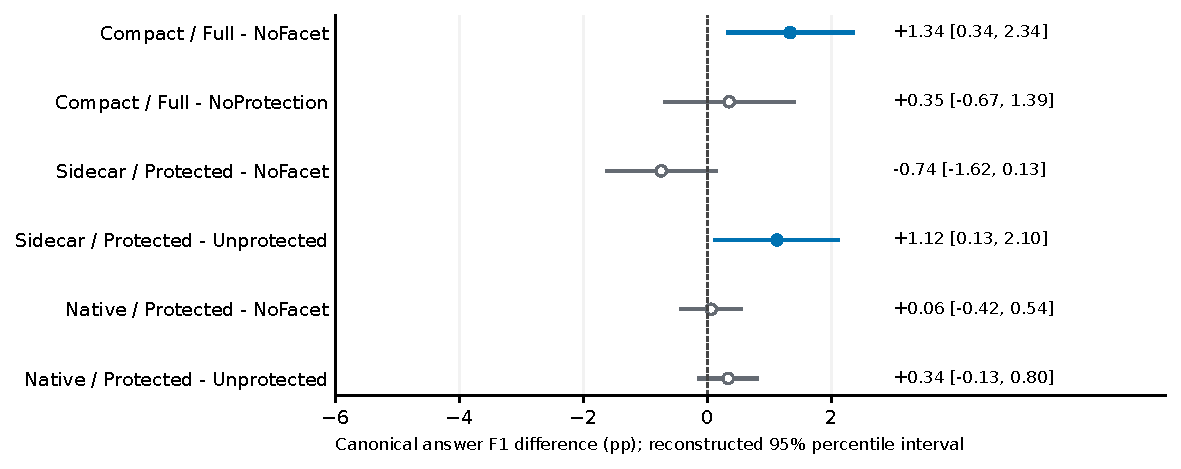
\includegraphics[width=\textwidth]{../shared/components.pdf}
\caption{Component and placement effects in percentage points, with recorded
95\% intervals, unchanged under canonical rescoring. Open markers cross zero.
Native NoFacet changes scoring coefficients in addition to facet eligibility,
so it is a pipeline comparison. The cross-space placement contrast has
verified identical prompt-visible evidence; this check is specific to that study.}
\label{fig:components}
\end{figure}

\subsection{Original Completion against a Stronger Baseline}
In the joint component set, BGE has answer F1 $.35801$ compared with
$.31803$ for original \full. The paired \full-minus-BGE difference is
$\effStrong$ $\ciStrong$, with its entire recorded interval below zero.
The original MiniLM-based system is therefore worse than BGE under that
evaluation. The gain over MiniLM cannot be substituted for an improvement
over a stronger retrieval backbone.

The same set gives \full-minus-BM25 $\effBm$ $\ciBm$ and
\full-minus-hybrid $\effHybrid$ $\ciHybrid$.
Both are unresolved. Including these reference points shows that the compact
gain is not a general win over all reasonable baselines.

\subsection{Cross-Space and Native BGE Extensions}
The sidecar tests complementarity while preserving BGE as the primary ranker.
Its Protected-minus-BGE effect is $\effSidecar$ $\ciSidecar$.
The native reconstruction yields $\effNative$ $\ciNative$ on its own
confirmation set. Neither establishes an increment. Their small negative
point estimates and intervals crossing zero do not demonstrate equality or
prove that every BGE-compatible structural method would fail.

\begin{table}[t]
\centering\small
\begin{tabular}{@{}llrrrr@{}}
\toprule
Evaluation & Method & F1 & EM & CR@20 & ER@20\\
\midrule
Joint component & BGE & .35801 & .30467 & .85400 & .93902\\
 & Original Full & .31803 & .26400 & .72217 & .87657\\
Cross-space & BGE & .34301 & .28000 & .84967 & .93594\\
 & Protected & .34045 & .27767 & .84350 & .93459\\
Native confirmation & BGE & .34569 & .28500 & .86167 & .94288\\
 & Protected & .34264 & .28133 & .86233 & .94288\\
\bottomrule
\end{tabular}
\caption{Absolute strong-backbone results under dataset-canonical scoring, averaged
equally across datasets within each evaluation. Different evaluation sets
are not pooled. The identical rounded native ER@20 values do not imply
identity of evidence sets.}
\label{tab:strong}
\end{table}

The native dataset-specific F1 differences are as follows:
\begin{align*}
\text{HotpotQA:}\quad &-.002907\quad [-.008682,.002652],\\
\text{MuSiQue:}\quad &-.003184\quad [-.008486,.001863].
\end{align*}
The equal-weight EM difference is $-.003667$, with an interval of
$[-.007667,.000004]$. These values corroborate the direction
of the reported point estimates but do not resolve either dataset-specific
comparison. The positive development value used to choose C10 is not
confirmation evidence.

The unprotected policies are informative additional references. Sidecar
Unprotected minus BGE is $\effSidecarUnprotected$
$\ciSidecarUnprotected$; native Unprotected minus BGE is
$\effNativeUnprotected$ $\ciNativeUnprotected$.
Both intervals lie below zero. Protection can reduce harm from an
intervention even when the protected intervention does not exceed the
original BGE baseline.

\subsection{Generator Transfer}
The pre-specified Gemma mobile-QAT deployment gives an equal-weight
\full-minus-Dense F1 effect of $\effGemma$ $\ciGemma$.
This result is unresolved. It is one additional generator configuration,
not evidence of universal transfer or an intrinsic architecture ranking.
Its reuse of initial rankings preserves the retrieval comparison, but does
not add new candidate-selection boundaries.

\begin{figure}[t]
\centering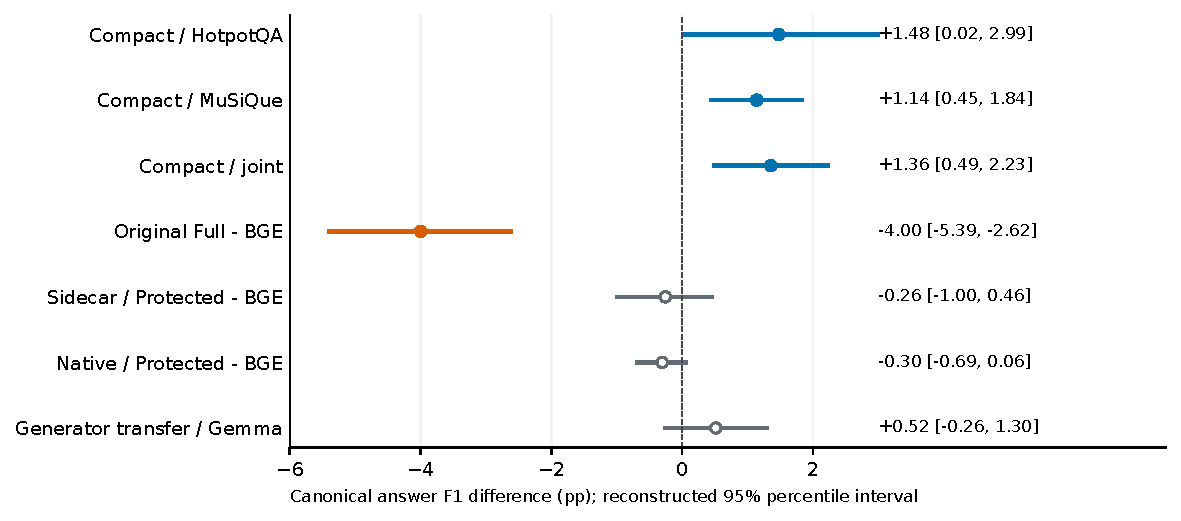
\includegraphics[width=\textwidth]{../shared/effects.pdf}
\caption{Main paired effects on a common percentage-point display scale.
The three compact rows, original-versus-BGE, two BGE extensions, and generator
transfer remain separate estimands. Lines are recorded 95\% percentile
intervals. This is not a fitted relationship between retriever strength and
benefit.}
\label{fig:effects}
\end{figure}

\section{Evidence Turnover, Cases, and Cost}
\subsection{A Fixed-Visible-Evidence Placement Comparison}
Write the BGE list as $D=(d_1,\ldots,d_K)$ and the insertion sequence as
$I$, with $m=|I|\leq4$. For $K=20$, $I\cap D=\varnothing$ and protected
prefix ten, the two orders are
\begin{align*}
R_P&=[d_1,\ldots,d_{10},I,d_{11},\ldots,d_{20}]_{:20},\\
R_U&=[I,d_1,\ldots,d_{20}]_{:20}.
\end{align*}
Since $20-m\geq10$, both contain exactly
$I\cup\{d_1,\ldots,d_{20-m}\}$. When fewer than twenty candidates exist,
the baseline already covers the universe and eligible outside-list insertions
are empty. This argument is specific to these constraints.

Independent reconstruction verifies these premises for every cross-space
question: 1,000 HotpotQA and 1,500 MuSiQue cases have identical final members.
It also rebuilds each arm's actual serialized prompt from the bound question,
unit titles and texts, template, and local tokenizer. All 5,000 prompt hashes
and token counts match their own recorded values. All 2,500 pairs retain the
same visible evidence IDs and text multiset, with no dropped or partially
truncated unit. Twelve HotpotQA questions have $K<20$ and no insertions.
Ordering changes for 458 HotpotQA and 1,070 MuSiQue questions; the remaining
pairs have identical prompts. The primary effect averages all queries.

The cross-space contrast is therefore an ordering/placement-policy comparison
at fixed visible evidence content, including the accompanying position
numbers. It does not reveal an internal attention mechanism. The positive
Protected-minus-Unprotected estimate coexists with an unresolved
Protected-minus-BGE estimate because the latter changes the evidence set.

\subsection{Entry Budget and Token Utilization}
The twenty-entry bound constrains membership; the 4,096-token cap bounds
serialized input length. Table~\ref{tab:tokens} distinguishes them using
actual per-query audits, not equality of aggregate averages.
\begin{table}[t]
\centering\small
\begin{tabular}{@{}lrrrrr@{}}
\toprule
Sidecar dataset & Min & Median & p95 & Max & At cap\\
\midrule
HotpotQA & 184 & 923.5 & 1,156.0 & 1,907 & 0/1,000\\
MuSiQue & 504 & 884.0 & 1,186.1 & 2,881 & 0/1,500\\
\bottomrule
\end{tabular}
\caption{Serialized input tokens for Protected and Unprotected. Counts are
identical within every paired query, not merely on average. Both arms have
zero evidence drops and zero partial truncations. The cap is 4,096 tokens.}
\label{tab:tokens}
\end{table}

The two sidecar orderings have identical token counts for each question, and
none reaches the cap. Across all 74,750 historical main prediction/prompt
pairs reviewed, including native development, the audits record zero
whole-unit drops and zero rank-one partial truncations. Thus, list-level
displacement in these runs should not be described as token-capacity
exhaustion. This observation does not imply that longer contexts would never
truncate or that equal entry budgets imply equal token costs across methods.

\subsection{Candidate Placement Is Not Uniform across Systems}
The existing Gold-free descriptive trace summaries show different intervention
rates. Under dataset-equal weighting, zero candidates are placed for 30.67\%
of compact queries, 41.43\% of sidecar queries, and 80.80\% of native queries.
Four candidates are placed for 33.95\%, 17.80\%, and 9.32\%, respectively
(Figure~\ref{fig:mechanisms}). These percentages describe distinct query sets
and distinct candidate rules; they are not the results of a matched
intervention-rate experiment.

The sparse native intervention gives context to its small aggregate effect.
Many queries preserve the original BGE ranking, while the modified queries
still need candidates that improve the answer. A lower intervention rate can
reduce both gain and harm. The trace does not establish whether the native
gates are too strict, whether available candidates are unhelpful, or whether
the generator fails to use them. Relaxing those gates after observing
confirmation would be a new selection decision, not further analysis of the
same frozen method.

\subsection{Supporting-Evidence Addition and Displacement}
The post-decision audits compare support identities entering and leaving
the final ranking. Sidecar HotpotQA has 21 added and 29 displaced supporting
units, for net $-8$. Sidecar MuSiQue has 59 added and 50 displaced,
for net $+9$. Native HotpotQA has 3 added and 2 displaced, while native
MuSiQue has 16 added and 15 displaced, giving net $+1$ in each.
Table~\ref{tab:turnover} preserves these totals and their denominators.

\begin{table}[t]
\centering\small
\begin{tabular}{@{}llrrrr@{}}
\toprule
Variant & Dataset & Questions & Added & Displaced & Net\\
\midrule
Sidecar & HotpotQA & 1,000 & 21 & 29 & $-8$\\
Sidecar & MuSiQue & 1,500 & 59 & 50 & $+9$\\
Native & HotpotQA & 1,000 & 3 & 2 & $+1$\\
Native & MuSiQue & 1,500 & 16 & 15 & $+1$\\
\bottomrule
\end{tabular}
\caption{Existing post-decision supporting-evidence events for Protected
relative to BGE. Counts use each dataset's support identities, so a MuSiQue
supporting paragraph is not a HotpotQA supporting sentence. These are
descriptive totals, not causal effect estimates or new confirmation tests.}
\label{tab:turnover}
\end{table}

\begin{figure}[t]
\centering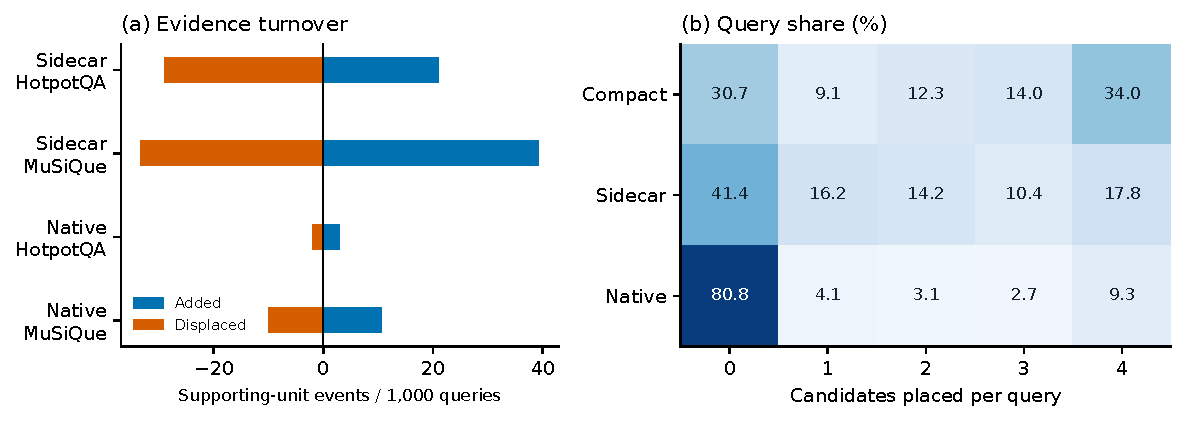
\includegraphics[width=\textwidth]{../shared/mechanisms.pdf}
\caption{Existing descriptive mechanism summaries. Left: added and displaced
annotated evidence per 1,000 questions, with direction represented by sign.
Right: dataset-equal-weight query percentages by placed-candidate count.
Candidate placement can include within-Top-20 promotion in the compact
variant; it is not interchangeable with genuinely new evidence.}
\label{fig:mechanisms}
\end{figure}

These counts do not yield a monotone account of answer utility. The native
system adds slightly more supporting evidence than it removes, yet both
dataset-specific answer-F1 point estimates are negative. An added supporting
unit may be redundant with retained text, and a displaced unit may have a
different role from an added one. Context order can also change what the
generator uses. No truncation was observed in the reviewed prompts, and the
fixed-content sidecar contrast separately estimates its placement-policy
effect. The turnover totals alone still do not identify mediation by any
particular added or displaced unit.

The practical implication is to report four objects separately: group-level
facet coverage, selected-unit coverage, prompt-visible evidence, and answers.
Only the last supplies the present primary endpoint. Treating an improvement
in the first as a guarantee about the last would overlook both displacement
and generation.

\subsection{Representative Success and Failure}
The existing qualitative selection uses the example closest to the median
answer-F1 change within a specified event family, with a stable identity
tie-break. The success family requires a positive compact Full-minus-Dense
answer change, improved complete recall, and an inserted supporting unit.
The failure family requires a negative original-Full-minus-BGE answer change
and a displaced supporting unit. This procedure selects illustrations after
the outcome; it does not create an unbiased estimate of prevalence.

The success question asks which film by the director of \emph{You and I}
concerns the Khmer Rouge. Dense retrieves a description of \emph{The Killing
Fields} at rank nine but answers \texttt{UNKNOWN}. Completion adds, at rank
twelve, a sentence about \emph{You and I} that identifies Roland Joff\'e and
connects him with \emph{The Killing Fields}. The generated answer changes to
the reference film, with F1 moving from zero to one.
The added bridge makes the answer derivable from the displayed evidence,
although one example cannot isolate a general causal mechanism.

The failure question asks whom the chairman of the Red Cross Aid to Russia
Fund was married to. BGE retains a rank-two sentence identifying Clementine
Churchill as Winston Churchill's wife and answers correctly. The original
compact Full ranking omits that supporting sentence and produces
\texttt{UNKNOWN}; its added sentence about a different Red Cross society
does not repair the link. This is a comparison of different retrieval
pipelines, not an instance of the protected sidecar evicting BGE's protected
rank-two unit.

\begin{table}[t]
\centering\small
\begin{tabular}{@{}p{.18\textwidth}p{.35\textwidth}p{.36\textwidth}@{}}
\toprule
Case & Evidence relation & Answer transition\\
\midrule
Compact success & Existing Khmer Rouge film description plus an added
director--film bridge & Dense: UNKNOWN $\rightarrow$ Full: The Killing
Fields; F1 $0\rightarrow1$\\
Cross-backbone failure & BGE marital relation omitted by original compact
Full; unrelated society sentence added & BGE: Sir Winston Churchill
$\rightarrow$ original Full: UNKNOWN; F1 $1\rightarrow0$\\
\bottomrule
\end{tabular}
\caption{Paraphrased illustrations from the existing representative-case
records. The second case is not a protected-placement ablation. Original
questions, evidence text, method identities, and selection rules remain in
the shared source CSV.}
\label{tab:cases}
\end{table}

\subsection{Computational Cost and What Was Measured}
For $n=|U_q|$, embedding dimension $d$, maximum depth $H$, and $B$ leaf
balls, dense scoring and sorting cost $O(nd+n\log n)$. Recursive assignment
costs $O(Hnd)$ because every level processes at most all candidates.
Facet scoring and ordering contribute $O(n+Bd+B\log B)$ apart from
tokenization; bounded insertion is linear in the traversed candidate list.
Working storage is $O(nd+n+B)$. These bounds exclude encoder and generator
inference, which have different computational profiles.

The native confirmation efficiency record reports 8.544 seconds for retrieval
reconstruction and a 670,420,228-byte embedding cache. Generation totals are
887.650 seconds for BGE, 884.198 for Protected, 886.058 for NoFacet, and
888.282 for Unprotected. Peak GPU memory is 3.592 GiB. These measurements
describe a cached local transaction; they are not full index-construction
costs, uncached retrieval latency, or evidence of a stable speed advantage
from a few seconds of timing difference.
The runner accumulates per-call generation seconds already stored in its
checkpoint before adding resumed calls. Consequently, transaction generation
seconds and the final process wall time have different scopes; their mismatch
is not by itself a timing error.

\begin{table}[t]
\centering\small
\begin{tabular}{@{}p{.49\textwidth}rp{.25\textwidth}@{}}
\toprule
Recorded item & Value & Interpretation\\
\midrule
Retrieval reconstruction & 8.544 s & Cached native transaction\\
BGE generation & 887.650 s & Per-method aggregate\\
Protected native generation & 884.198 s & Per-method aggregate\\
Peak GPU memory & 3.592 GiB & Recorded hardware\\
Embedding cache & 670,420,228 bytes & Existing cache identity\\
Main transaction generation calls & 10,000 & Four arms $\times$ 2,500 queries\\
Generated in final recorded process & 2,000 & Resume-process counter\\
Recorded failed calls & 0 & Historical telemetry\\
\bottomrule
\end{tabular}
\caption{Native confirmation cost record. Transaction-wide and final-process
counters are different fields; the table does not imply that 10,000 calls
occurred in the final resumed process. No generation was run for manuscript
preparation.}
\label{tab:cost}
\end{table}

Cache identity and deterministic subsets help interpret execution records,
but cache hits are not independent generated-answer reproductions. The
historical full or pre-selected subset rerun checks remain documented in
their original records. The present writing task does not rerun those
checks, infer new failure rates, or benchmark a repaired implementation.

\section{Discussion}
\subsection{What the Compact Gain Establishes}
The repeated compact differences demonstrate that an inference-time
completion layer can improve the tested MiniLM system without replacing
its encoder. The facet contrast further favors query-conditioned selection
over the specific centroid-only alternative. This is a meaningful result
about a constrained evidence-selection problem: a flat relevance list can
leave recoverable information outside the final context.

The comparison does not determine why granular-ball organization is the best
way to recover that information. Ordinary grouping, relevance--diversity
selection, and direct unit-level coverage could account for some or all of
the increment. The scalar compactness properties do not settle that
question, because they hold for arbitrary partitions. The appropriate
interpretation is therefore a useful complete pipeline plus limited
component evidence, rather than proof that every structural component is
irreducible.

\subsection{Interpreting the Strong-Backbone Boundary}
The BGE results change the practical claim. A user choosing between original
compact Full and BGE should not infer superiority from the MiniLM-relative
gain: the direct comparison favors BGE. The sidecar and native studies ask
whether structure can then complement that stronger reference. Their
intervals do not establish the desired increment.

One explanation is that BGE already retrieves much of the available useful
evidence, leaving fewer opportunities for completion. Other explanations are
poor candidate scoring, overly restrictive gates, insufficiently informative
lexical facets, or a mismatch between the selector and generator.
The existing comparisons do not identify which explanation dominates.
Because both algorithm definitions and query sets vary, a universal law that
benefit decreases with retriever strength would exceed the evidence.

The negative original-versus-BGE result and unresolved extension results
also have different meanings. The former interval is wholly negative; the
latter permit small effects in either direction. Neither should be hidden
behind a single qualitative success/failure label.

\subsection{Selection and Placement Are Distinct Decisions}
Protected placement is preferable to front insertion in the cross-space
study, yet Protected does not improve on BGE. Thus, placement can make a
candidate intervention less damaging without validating the candidate set.
The native protection contrast remains unresolved, showing that the placement
finding is not automatically portable between representations.

The cross-space study satisfies the fixed-visible-content condition:
the retrospective per-question reconstruction verifies identical evidence
members and texts under both orderings. It therefore estimates the effect of
the tested ordering/placement policy, including the associated position
numbers in the prompt. It does not identify an internal attention mechanism.
A pure evidence-set intervention would instead hold placement fixed and
change the selected units; that is a different comparison. Neither finding
establishes that Protected improves upon the original BGE ranking.

\subsection{Implications for Future Matched Comparisons}
The smallest informative extension would compare completion rules on a fresh
compact boundary while matching candidate access, final $K$, protected
prefix, changed positions, genuinely new units, and token accounting.
Ordinary clusters should match the actual group count of each candidate
configuration; a random grouping can additionally match group-size
distribution. Pure component ablations should zero the designated
coefficient while leaving the others unchanged. Independently tuned
pipelines answer a separate question and should be reported separately.

Such a study would need a prospective development/confirmation split, a
minimum meaningful effect, a finite tuning budget, and stopping rules.
Formal uncertainty should follow a justified sampling model and null
hypothesis. These are requirements for a future experiment, not additional
results of this article. Corpus-scale retrieval and external structured
methods would additionally require aligned corpora, readers, and budgets.

\section{Limitations}
The evidence is restricted to closed candidates in two English multi-hop QA
benchmarks. We do not evaluate corpus reachability, ANN recall, index
storage, full-wiki answer quality, multilingual transfer, or unanswerable
questions. MuSiQue's paragraph-level support annotations cannot be
reinterpreted as sentence-level reasoning-chain labels. Query terms also
need not contain the bridge entity required for a multi-hop answer.

Only one compact and one strong backbone are evaluated, with one principal
generator and one additional deployment configuration. The results cannot
establish broad generator robustness or a continuous relation between
retriever capacity and completion utility. Training-release questions may
have appeared in generator pretraining; project-held-out selection does not
eliminate that possibility.

Several mechanism claims remain unidentified. The compact radius split
trigger is redundant, the selector is static, group facets may exceed
selected-unit facets, and the native NoFacet comparator changes multiple
weights. There is no completed matched flat-unit, ordinary-clustering,
MMR, or sentence-coverage experiment. The mathematical coverage bound
belongs to a distinct surrogate and supplies no guarantee for historical
answer F1.

The measured scoring discrepancy is confined to one development question
and leaves the reported method differences unchanged. Historical
tail-probability calibration and source-document
dependence limit inferential claims. We do not silently replace the
historical statistics with a new test. The confidence intervals are not
equivalence bounds or uncertainty over model-development decisions.
Mechanism audits and qualitative examples are post-decision descriptions,
not new causal tests.

\section{Conclusion}
\hgrag frames structured evidence completion as a bounded intervention over
a dense retrieval ranking. The historical compact implementation repeatedly
improves MiniLM answer F1 in the evaluated closed-candidate settings, and
facet-conditioned selection exceeds its specified compact centroid-only
control. The original system nevertheless falls below BGE, and the tested
cross-space and native extensions do not establish an increment over BGE.
Protected placement reduces harm relative to front insertion in one
cross-space setting without establishing the usefulness of the intervention
against the untouched baseline.

The analysis explains why these outcomes are compatible. Group compactness,
lexical coverage, candidate addition, prompt-visible evidence, and answer
quality are different quantities. A method can improve one without
improving the next. Precise algorithm versions and matched comparisons are
therefore essential to attributing a gain. The existing evidence supports
completion for the tested compact system and motivates a narrower,
testable question about which candidate interventions can complement strong
retrieval.

\section*{Ethics, Availability, and Research Responsibility}
The study uses existing benchmark releases and documented model artifacts;
no new participant study is introduced. Positive, negative, and unresolved
results are retained. Third-party data and weights remain governed by their
original terms. The research repository contains implementations, frozen
derived records, and source data for the reported figures. An anonymous
artifact distribution and final reuse-license statement remain matters for
the human authors before submission.

AI tools assisted software work, analysis preparation, and manuscript
writing. They are not authors and do not bear responsibility for the work.
Human authors must confirm authorship, affiliations, funding, conflicts,
and the final venue-specific disclosure. No unconfirmed declaration is
inferred here.

\bibliographystyle{../shared/acl_natbib}
\bibliography{../shared/references}
\appendix
\section{Historical Evidence Mapping}
\label{app:scoring}
The paper's scientific comparisons correspond to the following internal
records: initial compact HotpotQA and MuSiQue are Stage4E and Stage4F;
generator transfer is Stage4G; joint components are Stage4H; the cross-space
sidecar is Stage4I; and native confirmation is Stage5A. These identifiers
are provenance labels, not the scientific organization of the argument.
The shared manuscript ledger lists the exact aggregate paths, effect
values, and historical-method interpretation.

\begin{samepage}
The baseline repository commit for the preceding audit was:
\begin{quote}\small\ttfamily
8a8e7cef8551c14bcea99e6a41a2b5a83f65456f
\end{quote}
\end{samepage}
The old PDF and source are retained separately from this manuscript version.
Some aggregate files retain a pending-verification status because verification
was written to a separate final artifact; the aggregation file is not
rewritten to erase that transaction history.

Later Stage6 development artifacts, its partially prepared official pipeline,
and the repaired v2 synthetic prototypes are not included in the empirical
tables. Their mathematical counterexamples help delimit possible claims,
but their synthetic behavior is not evidence about held-out answer quality.
No restricted reservation or Stage3B data is used in this manuscript revision.

\paragraph{Scorer sources and reconstruction.}
HotpotQA uses the official \texttt{hotpot\_evaluate\_v1.py} at revision
\texttt{3635853403a8735609ee997664e1528f4480762a}; MuSiQue uses
\texttt{metrics/answer.py} at revision
\texttt{922ac98f19a201998dbdae6d7f2887a5258dbdeb}. The revision package records
their source URLs and SHA-256 values and executes their reviewed pure answer
functions. Gold files match the historical frozen identities before parsing.
Per-query legacy values, all method means, original confirmation percentile
intervals, and generator-interaction intervals are reconstructed independently.
Legacy and canonical scores use exactly the same resampling draws. The
17 affected development predictions all belong to the same question; their
common F1 correction cancels in every within-query method contrast. Raw
reference maps are not distributed with the revision package.

The independent check addresses numerical scoring and prompt composition.
It neither certifies unrelated later verifier repairs nor supplies a
null-calibration proof for archived bootstrap-tail/Holm decisions.

\section{Terminology and Reporting Units}
\begin{longtable}{@{}p{.27\textwidth}p{.65\textwidth}@{}}
\toprule
Term & Meaning used in this article\\
\midrule
\endhead
Evidence completion & Bounded change to an existing evidence list; no promise
of complete reasoning support.\\
Granular ball & Local embedding group with a computed center and radius;
historical compact split eligibility is not independently radius-triggered.\\
Facet & Fixed-tokenizer query term occurring in a group's title/sentence union,
not a verified semantic subquestion.\\
Facet hyperedge & Seed-to-expansion group relation based on seed-relative
facet novelty and frozen gates.\\
Protected prefix & Initial dense entries preserved in order by the placement rule.\\
Placed candidate & Candidate accepted into the insertion segment; may be a
promotion from dense ranks 11--20 in the compact method.\\
Genuinely new unit & Unit in the completed list but absent from the baseline Top-20.\\
Evidence coverage & Coverage of annotated supporting identities at the
dataset's sentence or paragraph granularity.\\
Answer utility & Observed change in answer EM/F1, not a score used by the
confirmation retriever.\\
Unresolved effect & Recorded interval crosses zero; not evidence of equivalence.\\
Legacy scoring & Frozen evaluator used to reconstruct historical values;
the component, sidecar, and native versions lack HotpotQA's special-answer rule.\\
Canonical answer scoring & Dataset-specific official answer functions applied
retrospectively to unchanged predictions and verified reference files.\\
\bottomrule
\end{longtable}
\section{Counterexamples for Unevaluated Extensions}
A two-group activation objective illustrates a limitation of possible
extensions. For $e=\{a,b\}$, let $H(S)=\mathbf{1}[|S\cap e|\geq2]$.
Adding $b$ to the empty set has gain zero, while adding it to $\{a\}$ has gain
one, violating diminishing returns. Complementarity can be desirable without
being submodular.

Degree normalization presents a separate issue. Take hyperedges
$\{a,b\}$ and $\{b,c\}$, and divide newly activated edges by the incoming
group's degree. The path $a\rightarrow b$ accumulates $1/2$, whereas
$b\rightarrow a$ accumulates $1$ for the same final set $\{a,b\}$.
Such scores cannot be exact marginals of an order-independent set potential.
These are not the rules of historical compact q25. They supply no evidence
about its measured gains and no new empirical contribution. A bounded
lookahead alternative would require its own objective and cost evaluation.

\section{Reproduction Details}
\label{app:reproduction}
\paragraph{Retrieval and units.}
The compact encoder is \texttt{all-MiniLM-L6-v2}, with attention-mask mean
pooling, L2 normalization, and a 192-token encoder limit. BGE uses
\texttt{bge-large-en-v1.5}, CLS pooling, L2 normalization, and a 512-token
encoder limit. Its query instruction is ``Represent this sentence for
searching relevant passages:'' followed by the question. Document inputs
concatenate the title and sentence. HotpotQA preserves the supplied sentence
boundaries; MuSiQue splits whitespace-normalized paragraphs with the frozen
punctuation-and-capitalization rule. Neither splitter is changed in this review.
The reproducibility configuration pins the encoder revisions and unit IDs.

\paragraph{Lexical baselines.}
BM25 uses lowercase alphanumeric tokens, $k_1=1.5$, and $b=0.75$ within each
query's candidate set. Its inverse document frequency is
$\log(1+(N-df+0.5)/(df+0.5))$. The hybrid baseline averages query-local
min--max-normalized dense and BM25 scores with equal weights; a constant
score vector maps to zero. Unit ID breaks score ties. These are local
closed-candidate baselines, not corpus-scale retrieval systems.

\paragraph{Generation and budgets.}
The principal reader is Qwen2.5-1.5B-Instruct in FP16, using greedy decoding,
one beam, batch size one, and at most 32 generated tokens. The full serialized
input, including the chat template, is capped at 4,096 tokens. The system
instruction is: ``Answer the question using only the provided evidence.
Return only the shortest final answer. If the evidence is insufficient,
return UNKNOWN.'' Evidence is rendered in rank order as numbered
title--sentence entries, followed by the question and ``Final answer:''.
The Qwen runner sets CPU/CUDA seeds to zero, uses one CPU thread, and
enables deterministic algorithms. The renderer admits whole units in order
until the cap; only an overlong first unit permits partial truncation.
The compact policy protects ten dense positions and places at most four
candidates under a final budget $K=\min(20,|U_q|)$. Its frozen q25 floor is
0.1957079917192459. BGE-native has its own recorded eligibility policy;
it is not retrospectively identified with compact static-q25.

\paragraph{Scoring and interpretation.}
The reanalysis fixes the original predictions and reference channel. It
executes the pure answer-metric functions from the pinned official HotpotQA
and MuSiQue implementations, with maximum-over-alias scoring only where
the dataset permits aliases. HotpotQA assigns zero token F1 to mismatched
\texttt{yes}/\texttt{no}/\texttt{noanswer} responses, and zero F1 when both
normalized strings are empty. MuSiQue's official token F1 assigns one to
the latter case and does not inherit HotpotQA's categorical exception.
The archived per-query scores, means, and paired percentile intervals are
first independently reconstructed. Canonical scores then reuse the same
10,000 bootstrap draws. This isolates scorer migration from statistical
redesign: no new confirmatory test, model selection, or independent
confirmation is claimed. Supporting-evidence coverage retains the
dataset's original sentence or paragraph granularity and is not a
complete-chain recovery metric.

\end{document}
